\documentclass[a4paper,english, 10pt, twoside]{article}
\usepackage[utf8]{inputenc}
\usepackage[T1]{fontenc}
\usepackage[english]{babel}
\usepackage{epsfig}
\usepackage{graphicx}
\usepackage{amsfonts, amssymb, amsmath}
\usepackage{listings}
\usepackage{float}	%force figures in place with command \begin{figure}[H]
%\usepackage{subfigure}
%\usepackage{verbatim}
%\usepackage{parskip}
%\usepackage{color}

%\usepackage[squaren]{SIunits}
\usepackage[top=2cm, bottom=2cm, left=2cm, right=2cm]{geometry}
%\usepackage[top=0.2cm, bottom=0.2cm, left=0.2cm, right=0.2cm]{geometry}
%\usepackage[top=0.5cm, bottom=0.5cm, left=0.5cm, right=0.5cm]{geometry}

% \usepackage{titlesec}
% \titleformat{\section}{\large\bfseries\color{black}}{\thesection }{1em}{ }
% \titleformat{\subsection}{\bfseries}{\thesubsection}{1em}{ }
% \titleformat{\subsubsection}{\bfseries}{\thesubsubsection}{1em}{ }


%opening
\title{Project 1, FYS4150}
\author{Fredrik E Pettersen\\ fredriep@student.matnat.uio.no}

\begin{document}

\maketitle

\begin{abstract}
In this project we will look at a simple linear second order differential equation.
\end{abstract}

\section*{About the problem}
In this project we will look at a typical differential equation from some sort of physical problem, namely:
$$
\frac{d^2y}{dx^2} + k^2(x)y(x) = f(x)
$$
Where $f$ is normally the inhomogenous term, or some sort of forced motion etc, and $k^2$ is a real function of x. A classical 
equation on this form arises from electromagnetism, Poisson's equation.The eletrostatical potential $\Phi$ is generated by a 
localized charge distribution $\rho(\mathbf{r})$. In three dimentions Poisson's equation reads
$$
\nabla^2\Phi = -4\pi \rho(\mathbf{r})
$$
Which by the assumptions of both $\Phi$ and $\rho$ beeing spherically symmetric can be rewritten as
$$
-u''(x) = f(x)
$$
Which, with the boundary conditions $u(0)=u(1)=0$, and $x\in(0,1)$, is what we will be looking at in this project.\\
$f(x)$ in this case has the form $f(x) = 100e^{-10x}$. As you will se in the section regarding analytic solutions
this equation has the solution $u(x) = 1-(1-e^{-10})x-e^{-10x}$

\section*{The algorithm}
We start off by discretizing the problem by introducing the following aproximation to the second derivative:
$$
-u''(x) \simeq -\frac{u(x-h)-2u(x)+u(x+h)}{h^2} = f(x)
$$
Or in a slightly more compact notation
$$
2u_{i} - u_{i-1} - u_{i+1} = h^2f_i
$$
If we start off imagining that our problem only consists of 4 descrete points in the interval $x\in(0,1)$ and conduct the
calculations by hand ourselves we are left with the following:
\begin{align*}
h^2f_1 &= 2u_1 -u_2 \\
h^2f_2 &= -u_1 + 2u_2 -u_3 \\
h^2f_3 &= -u_2 + 2u_3 -u_4 \\
h^2f_4 &= -u_3 +2u_4
\end{align*}
Which is also satisfied by the matrix equation
\begin{align*}
 \left( \begin{array}{cccc} 2&-1&0&0\\
         -1&2&-1&0\\
         0&-1&2&-1\\
         0&0&-1&2 \end{array}\right)
 \cdot \left(\begin{array}{c} u_1\\u_2\\u_3\\u_4 \end{array} \right)
 =h^2\left(\begin{array}{c} f_1\\f_2\\f_3\\f_4 \end{array} \right)
\end{align*}

From here it is straightforward to generalize the expression into an $N\times N$ expression.\\
We can solve this set of linear equations by doing a forward substitution, eliminating all elements below the diagonal of the 
matrix and then do a backwards substitution after that. This can be done in several different ways. Gaussian elimination, 
LU decomposition, singular value ($PDP^{-1}$) decomposition just to mention a few. However all theese algorithms will take 
something like $O(N^3)$ floating point operations (FLOPS), and in this case they will spend a lot of time multiplying by zero 
(or even worse, dividing by zero). \\
Storing an $N \times N$ matrix with double precision floating point numbers will take up $8N^2$ bytes in RAM. Seeing as my 
computer only has 8GB of RAM N will be limited to $N< \sqrt{10^9} \simeq 3.1*10^4$. Should we set $N = 3*10^4$ we will store
$N^2 = 9*10^8$ elements in the matrix A. Only the diagonal and the lines above and below the diagonal are non-zero, this 
calculates to roughly $3N = 9*10^4$ which makes up 0.1\textperthousand \  of the numbers stored in RAM. Clearly we can make this more 
efficient. If we instead of storing the entire matrix only store the non-zero elements in vectors, one with the diagonal and two 
with the above and below diagonal elements, we can reduce the amount of elements stored to $8*3*N = 24N$, allowing us to make N 
of order $10^8$. If we tweak the forward and backwards substitutions to fit with vectors in stead of matrices we will also reduce 
the number of FLOPS used.\\
We notice here that every differential equation on the above form with the above approximation of the second derivative will 
have same matrix, A. This means that we can make the algorithm more effective by not adressing the i'th element of the 
vectors a, b and c, but rather just use the coefficients directly, thus reducing computing time even further. Doing this also 
means that we will not need to store the vectors a,b and c, which means we save $8*3 = 24n$ bytes in RAM.

If we now look at the following part of the most efficient code we can work out the number of FLOPS needed to do the calculations.\\

%Insert algorithm part here
temp[i] = c/btemp; is one FLOP.\\
btemp = b + temp[i]; is one more FLOP.\\
v[i] = (f[i] +v[i-1])/btemp; is two FLOPS.\\
So this loop ``consumes'' four FLOPS each round. Next we do the backwards substitution:\\
v[i] -= temp[i+1]*v[i+1]; This is also two FLOPS.\\ \\

In total this algorithm takes 6n FLOPS which is really not bad compared to the LU decomposition which we know from the 
lecture notes takes $\frac{2}{3}n^3$ FLOPS and another $O(n^2)$ to do the forward and backwards substitution to solve the set of
equations. As another point of comparison we know that Gaussian elimination also takes some $\frac{2}{3}n^3$ FLOPS.

\section*{Source code}
To solve the above described problem I have created the following code. As you will see from the comments there are several 
ways to do the nececary calculations. The current version of my program is not quite as general as it could have been, but it
can handle a resolution of $N = 10^8$. Should one however find it nececary, one can swich to the more general version and change
the wheighting in the derivative, and thereby the approximation.

\lstinputlisting{proj1.cpp}
\section*{Analytic solution}
The differential equation $-u''(x) = 100e^{-10x}$ can actually be solved analytically by LaPlace transform as follows
\begin{align*}
 -u''(x) &= 100e^{-10x}\\
 -\mathcal{L}[u''(x)] &= \mathcal{L}[100e{-10x}]\\
 -s^2u(s) +su(0) + u'(0) &= \frac{100}{s+10}\\
 u(s) &= \frac{-100}{s^2(s+10)} + \frac{u'(0)}{s^2}\\
 u(x) = \mathcal{L}^{-1}[u(s)] &= \mathcal{L}^{-1}\left[\frac{-100}{s^2(s+10)} + \frac{u'(0)}{s^2}\right]\\
 u(x) &= 1-e^{-10x} -x -xu'(0)\\
 \text{to determine }&u'(0)\text{ we exploit the boundary conditions}\\
 u(1) = 1-e^{-10} -1 -u'(0) &= 0 \implies u'(0) = e^{-10}\\
 \implies u(x) &=  1-(1-e^{-10})x-e^{-10x}
\end{align*}
This is of course also what we compare our nummerical solution to in the ``results'' section.

To properly test the limitations of this algorithm we could try running it for a few different right hand sides which yield 
known solutions for $u(x)$ such as $f(x) = sin(x),-e^{-x}, cosh(x),...$. However, we do already know the solution of this equation, 
and so this comparison would only reveal whether the algorithm dislikes any particular functions. I did try it for $f(x) = a = 1.8$
which makes $u(x) = 1.8x^2$, and this worked perfectly.\\
\section*{Results}
I have listed results in the form of plots of the numerical and exact solution. There is also a table containing relative errors 
and runtimes, as well as a comparrason with the LU decomposition algorithm from ``Armadillo''. This table is found in the
``Stability and Precision'' section. As we se from figure 3, increasing N will not give any visual difference, but I included
the plots for as large N as MatLab could handle without to much trouble.
\begin{figure}[H]
\begin{center}
 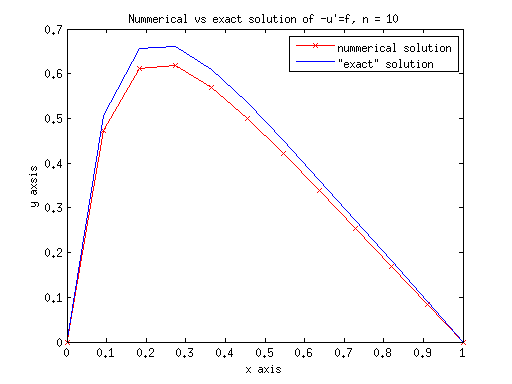
\includegraphics[scale=0.75]{plot_n10.png}\\
\caption{numerical and exact solution plotted with $n = 10$}
\end{center}
\end{figure}
\begin{figure}[H]
\begin{center}
 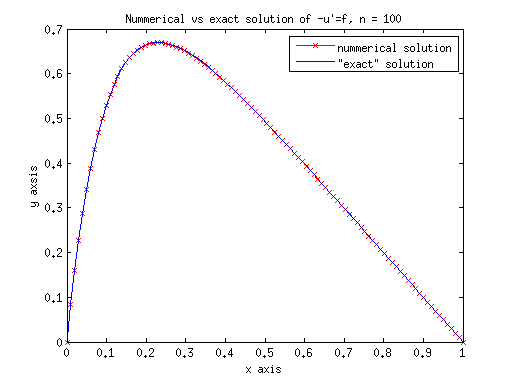
\includegraphics[scale=0.75]{plot_n100.png}\\
\caption{numerical and exact solution plotted with $n = 100$}
\end{center}
\end{figure}
\begin{figure}[H]
\begin{center}
 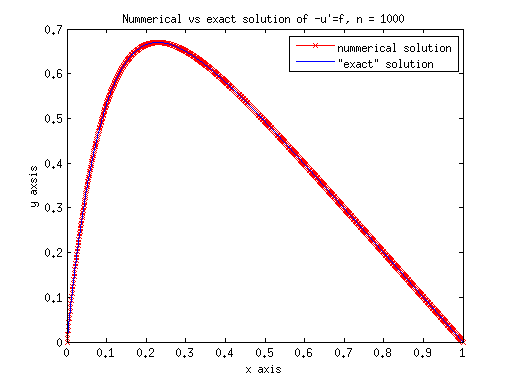
\includegraphics[scale=0.75]{plot_n1000.png}\\
\caption{numerical and exact solution plotted with $n = 1000$}
\end{center}
\end{figure}
\begin{figure}[H]
\begin{center}
 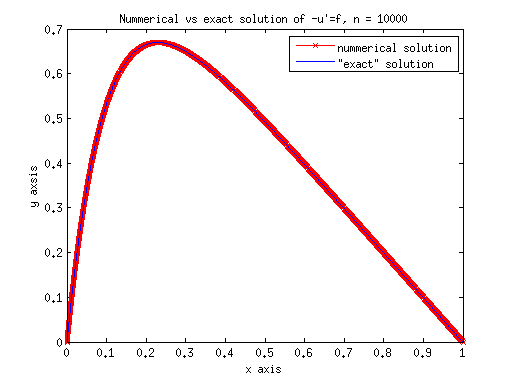
\includegraphics[scale=0.75]{plot_n10000.png}\\
\caption{numerical and exact solution plotted with $n = 10000$}
\end{center}
\end{figure}
\begin{figure}[H]
\begin{center}
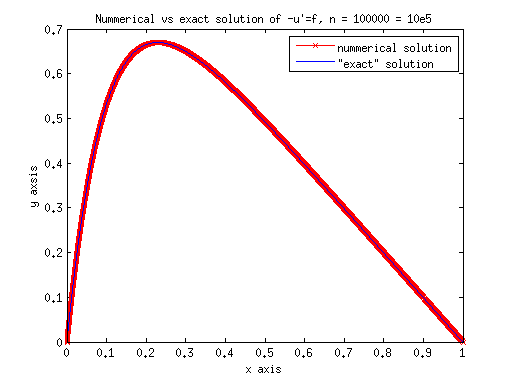
\includegraphics[scale=0.75]{plot_n100000.png}\\
\caption{numerical and exact solution plotted with $n = 100000$}
\end{center}
\end{figure}

\section*{Stability and precision}
To evaluate the precision of the algorithm derscribed above I have run the program a series of times with increasing N-values, and
calculated the maximum relative error to the exact solution. The results are listed in the table below. The relative error is 
calculated as follows.\\
$$
\epsilon_r = log10\left(abs\left(\frac{u_i - v_i}{u_i}\right)\right)
$$
All measurments of time are given in milliseconds and measured by the number of clock cycles the calculations required.
The relative error indicates how many decimals of precision we have in the numerical solution.\\

\begin{tabular}{|c|c|c|c|c|}
\hline
N & $\epsilon_r$ LU decomposition& CPU time LU decomposition &$\epsilon_r$& CPU time tridiagonal decomposition \\
\hline
5 & -12.5 & - & -0.7 & - \\
10 & ? & - & -1.2 & - \\
100 & -1.3 & - & -3.0 & - \\
500 & -1.9 & - & -4.4 & - \\
1000 & -2.2 & 30 & -4.8 & - \\
10000 & -3.2 & 3160 & -5.0 & - \\
$10^5$ & x & out of memory & -5.1 & - \\
$10^6$ & x & out of memory & -5.07 & 20 \\
$10^7$ & x & out of memory & x & 250 \\
$10^8$ & x & out of memory & x & 2380 \\
$1.5*10^8$ & x & out of memory & x & 3480 \\
\hline
\end{tabular} \\ \\


As we can clearly see, the error starts out quite large but over 2 orders of magnitude it decreases to an acceptable level of
five leading digits. As the table indicates, the error starts increasing again after $N = 10^5$. This is due to loss of 
numerical precision when $h^2 \to 10^{-15}$. The error in the LU - algorithm is sort of not working properly at this point because 
of the cheap fix I did when the backwards substitution could not access the first element in one of the vectors. 
\section*{Final comments}
The obvious conclusion we can draw from this project is that the custom made tridiagonal solver is much more efficient than the
more general solver based on LU decomposition. Not only is it faster, it can also work with a much finer resolution up to $10^8$
points. Of course in this exact problem the maximum resolution actually gives an increasing error, but should we increase the 
interval which $u(x)$ is defined on to say $x \in (0,100)$ (for some other $f(x)$) the value of $h^2$ will increase to $10^{-12}$
for $N = 10^8$, and we will benefit from the increased resolution.
I know that my program could have been structured better by making a header-file containing the different loops and initialization
of variables. I will try to improve on this.
\end{document}
